\documentclass[12pt,a4paper]{scrartcl}
\usepackage[utf8]{inputenc}
\usepackage[ngerman]{babel}
\usepackage{amsmath}
\usepackage{amsfonts}
\usepackage{amssymb}
\usepackage{color}
\usepackage{graphicx}
\usepackage{listings}
\usepackage[left=2.5cm, right=2cm, top=2cm, bottom=2cm]{geometry}

\usepackage[hidelinks]{hyperref}
\usepackage{scrpage2}
\usepackage{csquotes}
\usepackage{subcaption}


\DeclareUnicodeCharacter{00A0}{ }

\pagestyle{scrheadings}


\linespread{1.5}
\setlength{\parindent}{0cm} % No paragraph indent


\newcommand{\q}[1]{``#1''}
\newcommand{\todo}[1]{\begin{Large}\textcolor{red}{$\Rightarrow ~$#1}\end{Large}}

\newcommand{\ant}[1]{\begin{Large}\textcolor{green}{$\Rightarrow ~$#1}\end{Large}}


\newcommand{\inmilestonetwo}{\vspace{0.75cm} \framebox[1.1\width]{
\begin{large}
\textcolor{red}{Die Dokumentation dieses Abschnittes ist für Milestone II vorgesehen.}
\end{large}}}



\begin{document}

% University Assignment Title Page 
% LaTeX Template
% Version 1.0 (27/12/12)
%
% This template has been downloaded from:
% http://www.LaTeXTemplates.com
%
% Original author:
% WikiBooks (http://en.wikibooks.org/wiki/LaTeX/Title_Creation)
%
% License:
% CC BY-NC-SA 3.0 (http://creativecommons.org/licenses/by-nc-sa/3.0/)
% 

\begin{titlepage}

\newcommand{\HRule}{\rule{\linewidth}{0.5mm}} % Defines a new command for the horizontal lines, change thickness here

\center % Center everything on the page
 
%----------------------------------------------------------------------------------------
%	HEADING SECTIONS
%----------------------------------------------------------------------------------------

\textsc{\LARGE Programmierprojekt}\\[1.5cm] % Name of your university/college
\textsc{\Large Alte Kantonsschule Aarau}\\[0.5cm] % Major heading such as course name
\textsc{\large}\\[0.5cm] % Minor heading such as course title

%----------------------------------------------------------------------------------------
%	TITLE SECTION
%----------------------------------------------------------------------------------------

\HRule \\[0.4cm]
{ \huge \bfseries Dokumentation: Spacetraveler}\\[0.4cm] % Title of your document
\HRule \\[1.5cm]
 
%----------------------------------------------------------------------------------------
%	AUTHOR SECTION
%----------------------------------------------------------------------------------------

\begin{minipage}{0.4\textwidth}
\begin{flushleft} \large
\emph{Autoren:}\\
Gabriel \textsc{Gavrilas}\\ % Your name\\
Patrick \textsc{Eigensatz}\\ % Your name\\
Jonas \textsc{Wahlen}\\ % Your name\\
\end{flushleft}
\end{minipage}
~
\begin{minipage}{0.4\textwidth}
\begin{flushright} \large
%\emph{Betreuer:} \\
%Dr. Martin \textsc{Jordi} % Supervisor's Name
\end{flushright}
\end{minipage}\\[2cm]

% If you don't want a supervisor, uncomment the two lines below and remove the section above
%\Large \emph{Author:}\\
%John \textsc{Smith}\\[3cm] % Your name

%----------------------------------------------------------------------------------------
%	DATE SECTION
%----------------------------------------------------------------------------------------

{\large Februar 2016}\\[2cm] % Date, change the \today to a set date if you want to be precise

%----------------------------------------------------------------------------------------
%	LOGO SECTION
%----------------------------------------------------------------------------------------

%\includegraphics[width=12cm]{img/titelbild.jpg}\\[1cm] % Include a department/university logo - this will require the graphicx package
 
%----------------------------------------------------------------------------------------

\vfill % Fill the rest of the page with whitespace

\end{titlepage}

\clearpage

\tableofcontents

\clearpage

\todo{Informationen / Beispielarbeit beachten!}

\section{Projektbeschreibung}
\subsection{Spielidee}
Ziel unseres Spieles ist es, dass der Spieler sein Raumschiff von einer Startposition im Level
zum Ziel bringt. Dazu eine kleine Story:
\begin{quote}
Der verrückte Wissenschaftler Prof. Lewinsky war mit seiner Rakete auf der Suche nach einem äusserst seltenen Element welches er zur Fertigung seiner Gravitationskanone benötigt. 
In einer weit entfernten Galaxie wurde er Fündig. 
Beim Treibstoff hatte er sich jedoch verrechnet und stand nun ohne Antrieb am anderen Ende des Universums.
Glücklicherweise konnte er seine Gravitationskanone an Bord fertigstellen.
Deine Aufgabe ist es nun Prof. Lewinsky mithilfe der instabilen und ungetesteten Gravitationskanone nach Hause zu befördern. 
Dabei musst du auf die herumfliegenden Asteroiden achtgeben. 
Vor allem solltest du dich jedoch vor den abnormal kleinen Schwarzen Löchern in Acht nehmen, die nur in diesem Teil des Universums vorkommen und dich sofort anziehen, wenn du ihnen zu nahe kommst. 
Hilf dem hoffnungslosen Theoretiker nach Hause zu kommen!
\end{quote}

\subsection{Physik}
In unserem Spiel haben wir einige Elemente der Physik der realen Welt übernommen.
Dabei handelt es sich nur schon um Geschwindigkeit, Beschleunigung und Kräfte.
Dazu haben wir auch die Gravitation und den elastischen Stoss, als komplexere Vorgänge modelliert.
\subsubsection{Geschwindigkeit, Beschleunigung, Kraft}
Unser Spieler bewegt sich im Level.
Hier ist bereits die Sprache von Geschwindigkeit.
Zur Geschwindigkeit ist wohl keine Erklärung nötig.
Dazu kommt die Beschleunigung, die man als zeitliche Änderung der Geschwindigkeit auffassen kann.
Wichtig zu verstehen ist jedoch der Zusammenhang zwischen Kraft und Beschleunigung.
Um Kräfte zu berechnen nimmt man das Produkt aus Beschleunigung und Masse.
Also ist die Beschleunigung, wenn die Kraft bekannt ist, auch von dem Faktor Masse abhängig. ...

\subsection{Gravitation}
Unter Gravitation versteht man in der Physik, die Anziehngskraft, mit der sich Masse anzieht.
Bekannt ist uns die Gravitation von den Planeten und ihren Anziehungskräften.
Die Sonne zieht mit ihrer enormen Masse die Planeten an und die Planeten ziehen die Monde an.
Auf der Erde zeigt sich Gravitation als Schwerkraft, die uns am Boden hält.
Dies kommt davon, dass die Erde sehr viel grösser als wir ist.
Im Sonnensystem jedoch findet Gravitation zwischen Objekten ähnlicher Grösse statt.
Wenn sich ein Objekt einem anderen nähert gibt es drei Mögliche Auswirkungen.
\begin{enumerate}
\item Sie ziehen sich gegenseitig so an, dass sie miteinander kollidieren.
\item Sie sind schnell und lenken sich gegenseitig bei nahekommen einfach ab, entfernen sich danach jedoch zu weit um weiter Einfluss aufeinander zu bewirken.
\item 

\end{enumerate}


\subsection{Elastischer Stoss}
Im Spiel brauchen wir bei der Kollision der einzelnen Asteroiden und der Kollision mit der Wand das Prinzip des vollkommen elastischen Stosses. \\
In der realen Welt kommt es ständig zu Kollisionen, sei es ein Fuss, der auf einen Ball trifft, Billardkugeln die Kollidieren, oder zwei Autos bei einer Frontalkollision. 
Ständig stossen Objekte aufeinander. \\
Die Physik kennt verschiedene Arten solcher Stösse.
Unterschieden wird dabei, wie Energie übertragen wird.
Speziell im Bezug auf den Stoss sind das innere Energie und kinetische Energie.
Einfach gesagt unterscheidet man, ob sich Objekte bei einer Kollision verformen und/oder erhitzen, oder sie ihre Geschwindigkeit und Richtung ändern.\\
Die Extremfälle bilden also zum einen ein Stoss, bei dem Beide Objekte sofort still stehen und sich erwärmen oder deformieren.
Dies nennt man den vollkommen unelastischen Stoss.
Zum anderen ein Stoss, bei dem die Objekte keine Deformation oder Erwärmung erfahren, sondern eine Änderung der Geschwindigkeit und der Bewegungsrichtung stattfindet.
Dies nennt man den vollkommen elastischen Stoss.\\
Beide Fälle sind Idealfälle.
Sie kommen in der realen Welt nicht vor.
In unserem Spiel wollten wir einen beinahe vollkommen elastischen Stoss umsetzen.
% langet da? wo selli da wege vektorfällig schriibe im andere teil denne?




\section{Problemdefinition}
\subsection{Grundkriterien}
Wir haben uns folgende Grundkriterien gesetzt:
\begin{itemize}
\item Gravitation: Punkte, die den Spieler unterschiedlich stark gegen sich ziehen.
\item Der Spieler ist ein Raumschiff.
\item Der Spieler befindet sich in einem Raum fernab von jeder anderen Kraftquelle ausserhalb des Levels.
\item Der Spieler bewegt sich durch dieses Level mithilfe von  einem Gravitationspunkt, den er platzieren und entfernen kann; Er kann sich also \q{in eine Richtung ziehen lassen}
\item Das Level ist beschränkt, hat also einen Start und ein Ziel
\item Es gibt Wände, die den Raum beschränken.
\end{itemize}

\subsection{Zusatzkriterien}
Als Zusatzkriterien setzen wir uns weiter:
\begin{itemize}
\item Gegner und/oder Hindernisse (= Objekte bei deren Kollision der Spieler stirbt) z.B: Asteroiden die sich frei bewegen, oder sehr starke Gravitationszentren, die den Spieler gegen ein Objekt ziehen und so eine Kollision auslösen.
\item Gameover-Grafik, die angezeigt wird, wenn der Spieler stirbt oder die Zeit abläuft.
\item Es besteht eine kleine Reibung, die den Spieler leicht abbremst.
\item Zeitliche Beschränkung (z.B: 2min, wenn Zeit = 0, ist das Spiel zu Ende)
\item Startmenu und Spielanleitung
\end{itemize}




\section{Anforderungsanalyse}
% maximal 2 sätze, in java realisierbar
Das Programm lässt sich mitsamt seinen Anforderungen vollständig in Java implementieren.
Es werden auf Soft-/Hardwareebene keine weiteren Anforderungen gestellt, als ein einfacher Computer mit
Maus und funktionierender JRE.


\section{Spezifikation}
\subsection{Use Cases}
\subsubsection{Spieler}
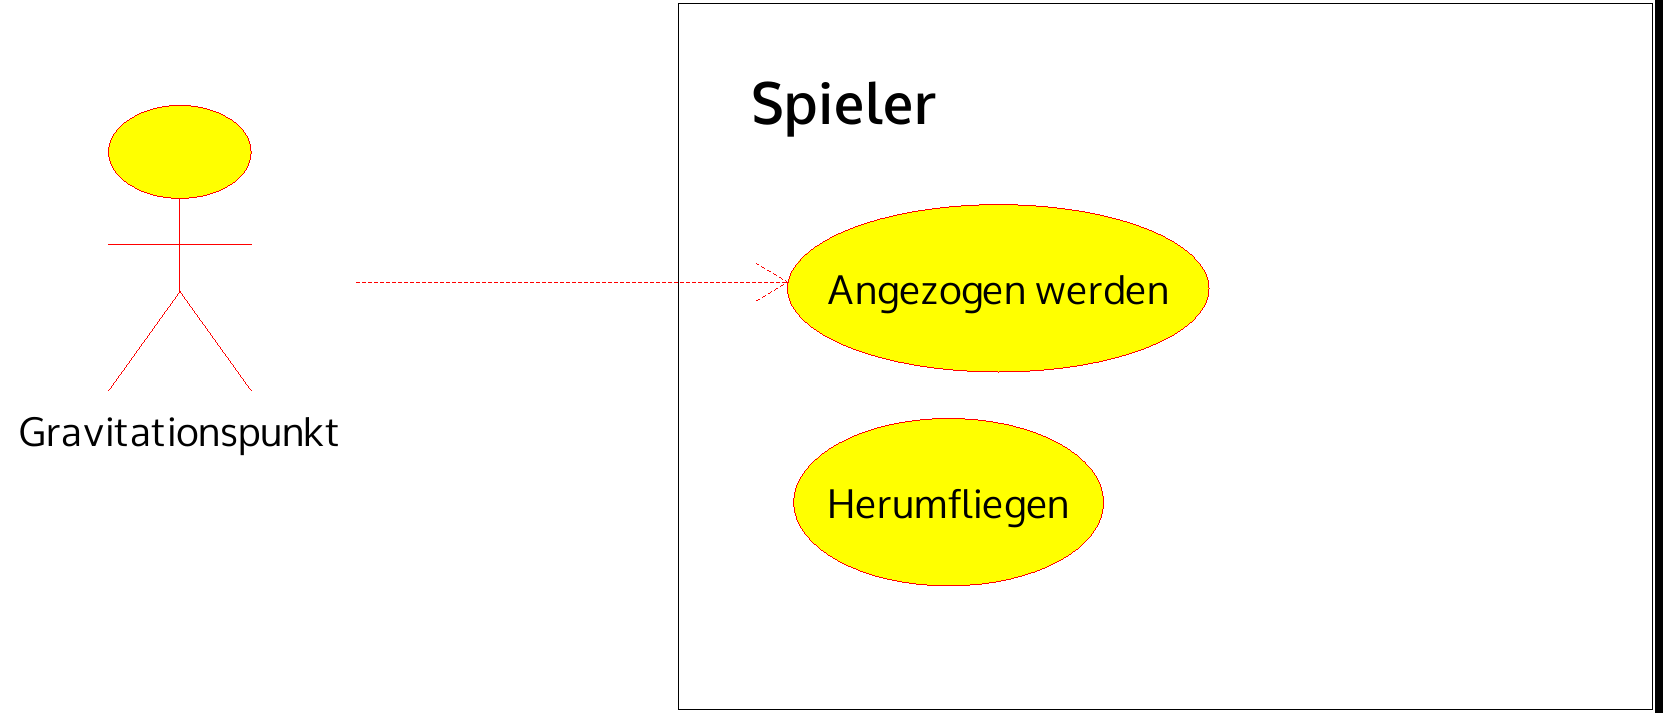
\includegraphics[scale=0.2]{use_cases/spieler.png}


\subsubsection{spaceObject}
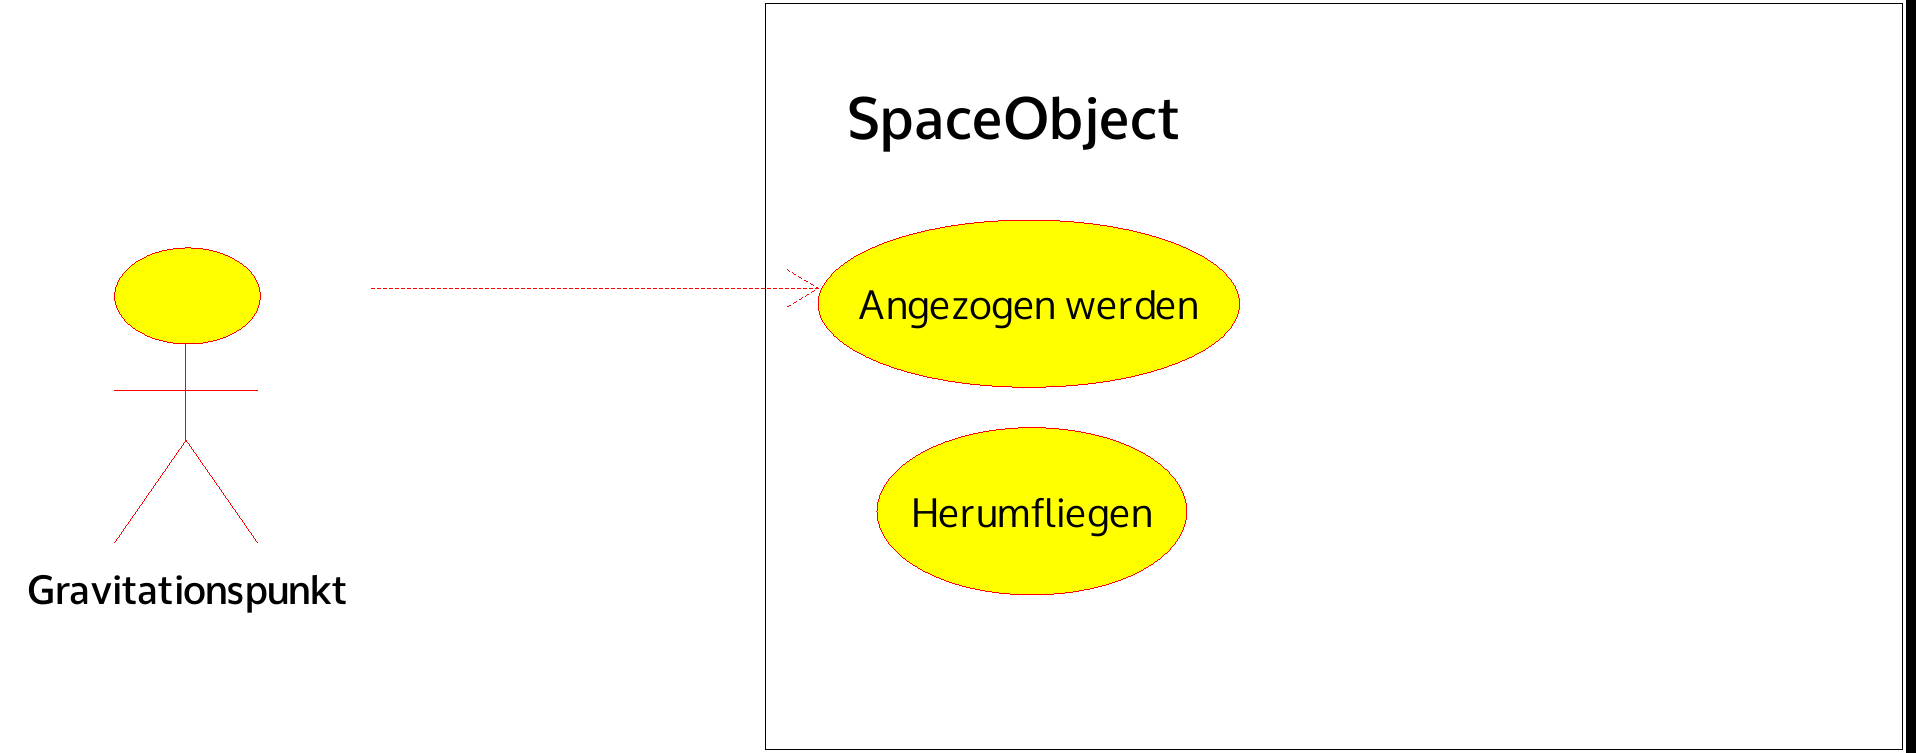
\includegraphics[scale=0.2]{use_cases/spaceObject.png}\\
Ein spaceObject kann von einem Actor (Gravitationspunkt) angezogen werden. Das spaceObject
\q{fliegt} aber jeder Zeit \q{herum}. Dazu braucht es keinen Actor.


\subsection{Anforderungen} 
\subsubsection{Technische Ausführung}
\begin{itemize}
\item Mit der Maus soll das Setzen eines Gravitationspunktes - und damit die Steuerung der Spielfigur - möglich sein.
\item Java packages: \begin{itemize}
	\item java.util.* \textit{(Datenstrukturen)}
	\item java.io.* \textit{(Um Daten aus dem .jar als Streams zu laden)}
\end{itemize}
\item JSFML packages: \begin{itemize}
	\item org.jsfml.Graphics.* \textit{(Grafik-API von JSFML)}
	\item ...
\end{itemize}
\end{itemize}
	%% technische ausführung

\subsection{Dokumentation}
Diese Dokumentation wurde in \LaTeX \. erstellt. Da die Quellcodedateien im Textformat und nicht
binär vorliegen konnten wir sie ebenfalls in unser Revisionskontrollsystem einbinden und parallel
an ihr schreiben.

Da wir unseren Code mit den entsprechenden Kommentaren ausgeschmückt haben,
konnten wir eine detaillierte Codedokumentation mit dem Programm \textit{doxygen} (ähnlich wie javadoc) erstellen lassen.
Die PDF-Datei, die dabei herauskam liess sich leicht an unsere Dokumentation anhängen.

Der Quellcode wurde über das \textit{listings}-Paket direkt von LaTeX selbst eingelesen und formatiert.

\subsubsection{Gravitation}
- Punkte die den Spieler unterschiedlich stark anziehen.
Im Rahmen der Implementierung der Gravitation haben wir die ganze Physik ins Spiel gebracht.
%gravityModel erklären

\subsubsection{Der Spieler ist ein Raumschiff}
Der Spieler steuert ein Raumschiff, indem er es von den beschrieben Gravitationspunkten in eine Richtung ziehen oder stossen lässt.\\

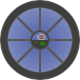
\includegraphics[scale=0.5]{img/spieler.png}


\subsubsection{Raum frei von auswärtigen Kräften}
% kurze erläuterung

\subsection{Spieler bewegen / Gravitationspunkt}
% hier spezifisch den punkt bei mausklick

\subsection{Level}
%tiles
\subsubsection{Start und Ziel}

\subsubsection{Wände}

\subsection{- Gegner und Hindernisse}
% Asteroiden und Schwarzes Loch

\subsection{- Gameover}

\subsection{- kleine Reibung}

\subsection{Zeit}

\subsection{Startmenu}

\subsection{Spielanleitung}


\clearpage
\newpage
\section{Entwurf}
\subsection{UML Diagramm}
\vspace{0.3cm}
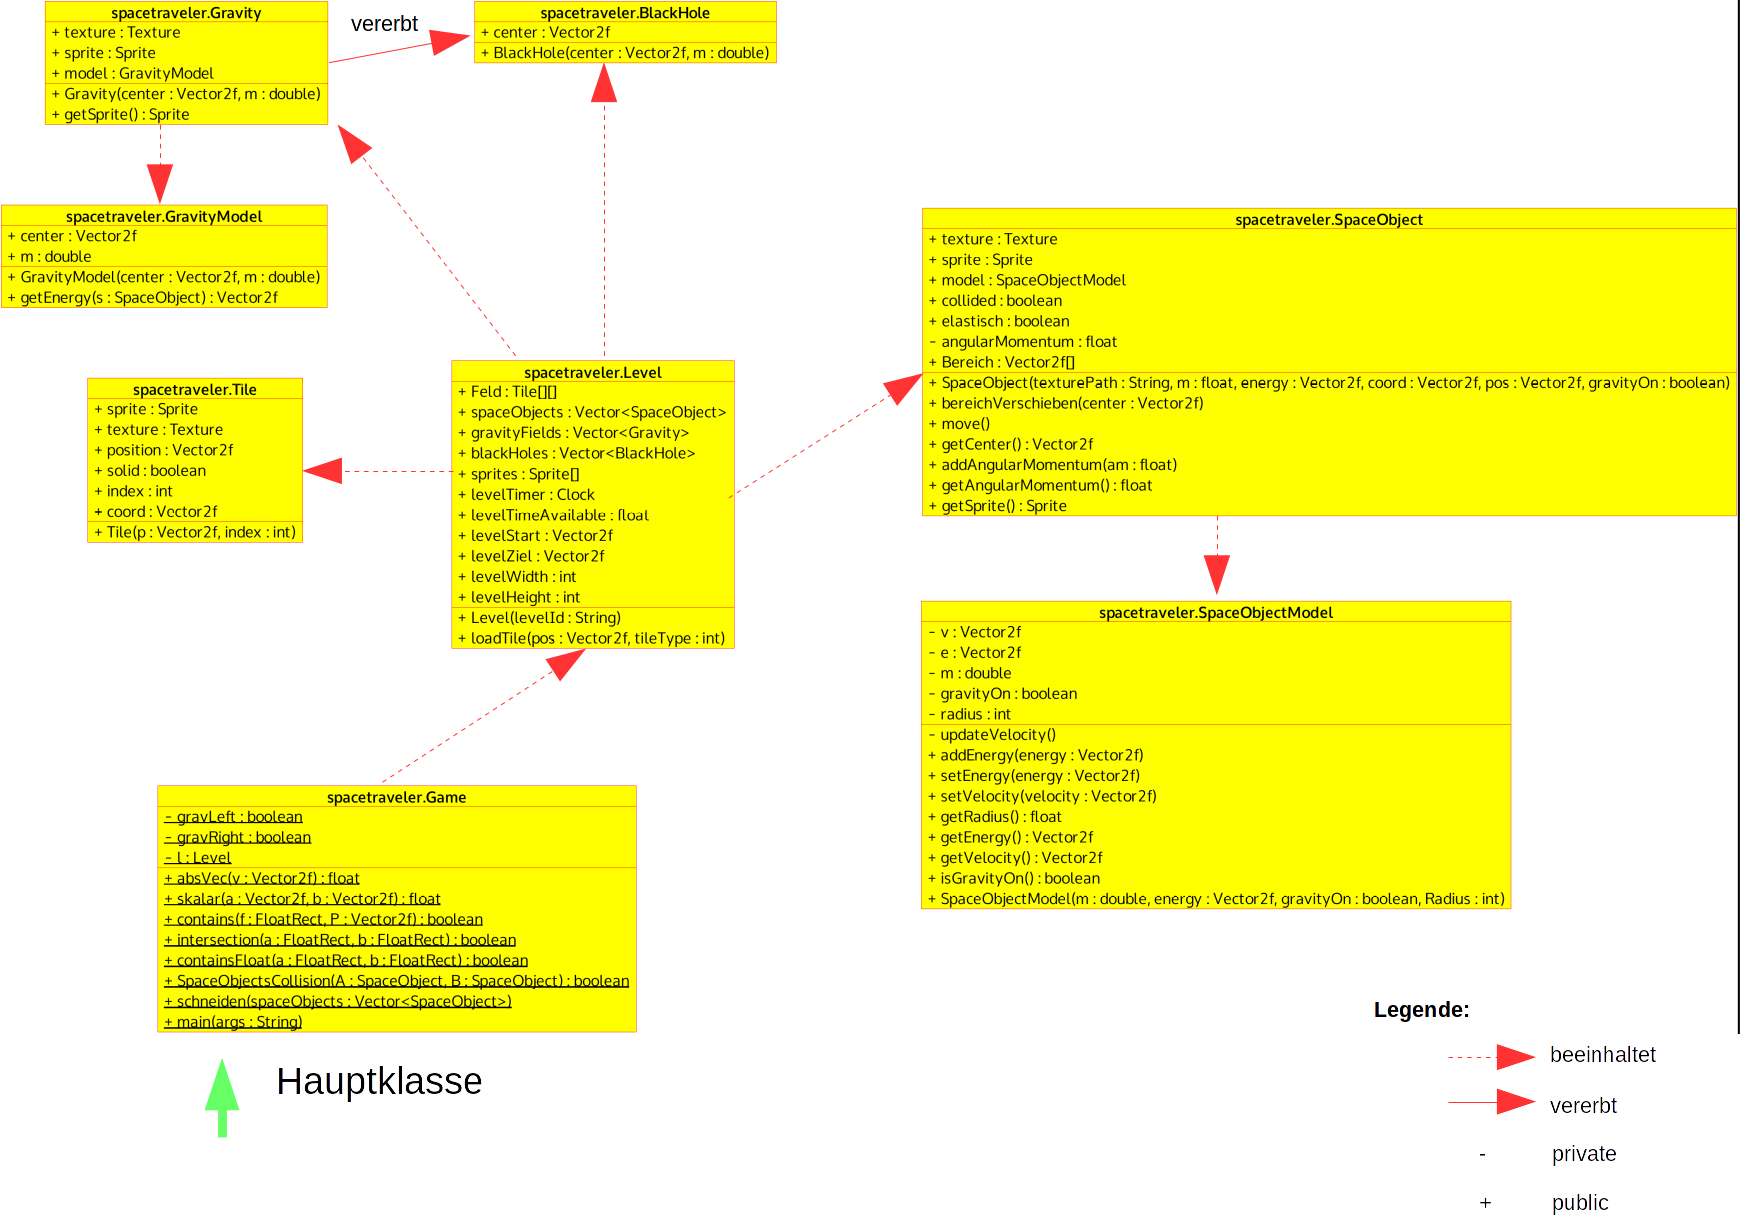
\includegraphics[height=0.85\textwidth,angle=90]{img/uml.png}

\section{Implementierung}
% Quellcode
\section{Quellcode}
\subsection{Über unseren Quellcode}
Unser Code ist modular aufgebaut, d.h. das Spiel besteht aus verschiedenen Klassen. Jede Klasse
verfügt über eine eigene Datei.
\subsection{Level.java}
\lstinputlisting[language=Java,breaklines=true,numbers=left,tabsize=4]{../../src/spacetraveler/Level.java}


\section{Resultate und Testen}
\inmilestonetwo
\section{Diskussion und Ausblick}
\inmilestonetwo




\end{document}
 
